\documentclass[aspectratio=169,unicode,dvipdfmx,14pt]{beamer}

\usepackage{url}
\usepackage{bm}
\usepackage{amsmath}
\usepackage{amssymb}
\usepackage{graphicx}
\usepackage[absolute,overlay]{textpos}
\usepackage{hyperref}
\usepackage{listings}

\usefonttheme[onlymath]{serif}

\DeclareMathOperator*{\argmax}{argmax}

\hypersetup{
	setpagesize=false,
	bookmarksnumbered=true,%
	bookmarksopen=true,%
	colorlinks=true,%
	linkcolor=blue,
	citecolor=red,
}

\newcommand\FontMath{\fontsize{10}{12}\selectfont}
\renewcommand{\baselinestretch}{1.3}
\renewcommand{\familydefault}{\sfdefault}
\renewcommand{\kanjifamilydefault}{\gtdefault}
\usepackage[deluxe, expert]{otf}

\setbeamertemplate{navigation symbols}{}
\setbeamertemplate{footline}[frame number]
\setbeamerfont{footline}{size={\fontsize{15}{15}}}

\setbeamerfont{author}{size=\Large}
\setbeamerfont{institute}{size=\normalsize\itshape}
\setbeamerfont{title}{size=\huge}
\setbeamerfont{subtitle}{size=\LARGE\normalfont\slshape}


\title{ \\二項分布}
\author{\texorpdfstring{正田 備也\newline\href{mailto:masada@rikkyo.ac.jp}{masada@rikkyo.ac.jp}}{正田 備也}}
\date{}

\begin{document}

\begin{frame}
\titlepage
\end{frame}

\section{ベルヌーイ分布と二項分布}

\begin{frame}\frametitle{Contents}
\Large \tableofcontents[currentsection]
\end{frame}

\begin{frame}{ベルヌーイ分布 Bernoulli distribution}
\begin{itemize}
\item $V=\{\mbox{v}_1,\mbox{v}_2\}$という2種類のアイテムの集合上に定義される確率分布
\begin{itemize}
\item 例えば、コインの表が$\mbox{v}_1$でコインの裏が$\mbox{v}_2$など
\end{itemize}
\item パラメータは$\bm{\phi} = (\phi_1, \phi_2)$
\begin{itemize}
\item アイテム$\mbox{v}_1$が出現する確率$\phi_1$
\item アイテム$\mbox{v}_2$が出現する確率$\phi_2$
\item $\phi_1 + \phi_2=1$が成り立つので、自由度は1
\item[] \
\item[] \
\end{itemize}
\end{itemize}
\begin{textblock*}{0.4\linewidth}(290pt, 110pt)
    \centering
    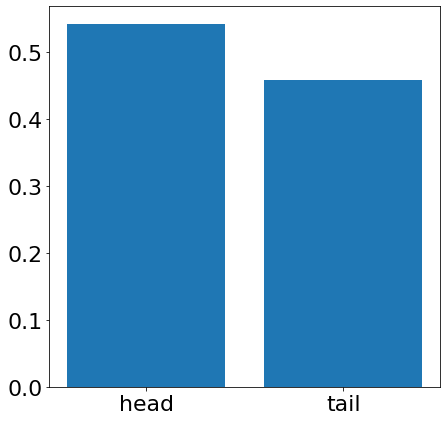
\includegraphics[width=0.8\linewidth]{bernoulli_bar}
\end{textblock*}
\end{frame}

\begin{frame}{二項分布 binomial distribution}
\begin{itemize}
\item 複数回のコイン投げのモデリングには二項分布を使う
\begin{itemize}
\item ベルヌーイ分布は1回のコイン投げのモデリングに使う
\end{itemize}
\item 試行回数を$n$として、``$n$回のうち$\mbox{v}_1$が$k$回出現する確率がこれこれ''というふうに、$k=0$から$k=n$までの、ありうる出現回数すべてに、確率を割り振る確率分布
\item パラメータは$n$と$\bm{\phi} = (\phi_1, \phi_2)$
\begin{itemize}
\item 試行の回数$n$(これは観測データから決まる)
\item アイテム$\mbox{v}_1$が出現する確率$\phi_1$
\item アイテム$\mbox{v}_2$が出現する確率$\phi_2$
\item $\phi_1 + \phi_2=1$が成り立つので、自由度は1
\end{itemize}
\end{itemize}
\begin{textblock*}{0.4\linewidth}(305pt, 150pt)
    \centering
    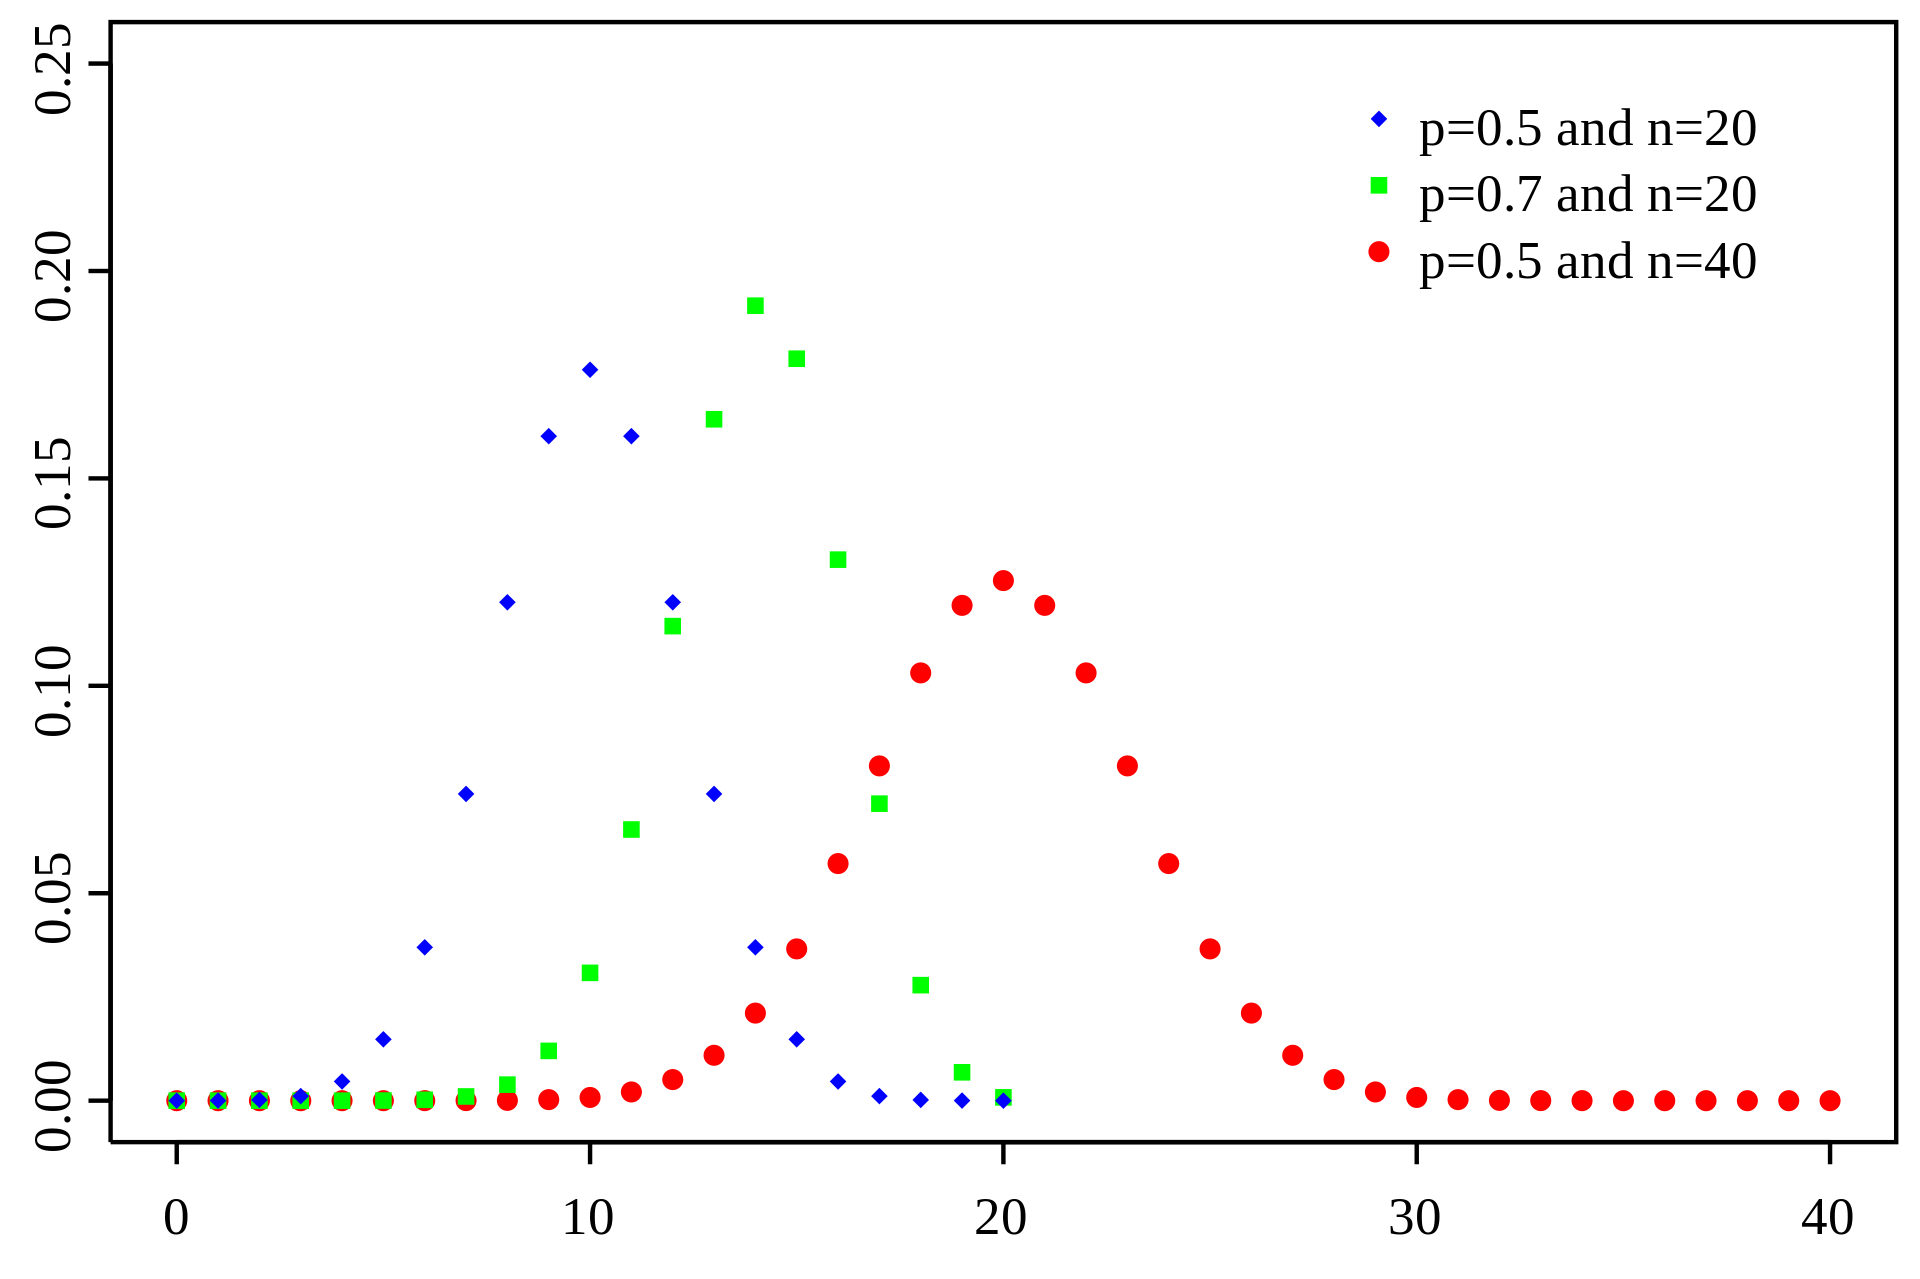
\includegraphics[width=0.8\linewidth]{1920px-Binomial_distribution_pmf.svg}
\end{textblock*}
\end{frame}

\begin{frame}
\begin{figure}[htbp]
\begin{center}
\vspace{.2in}
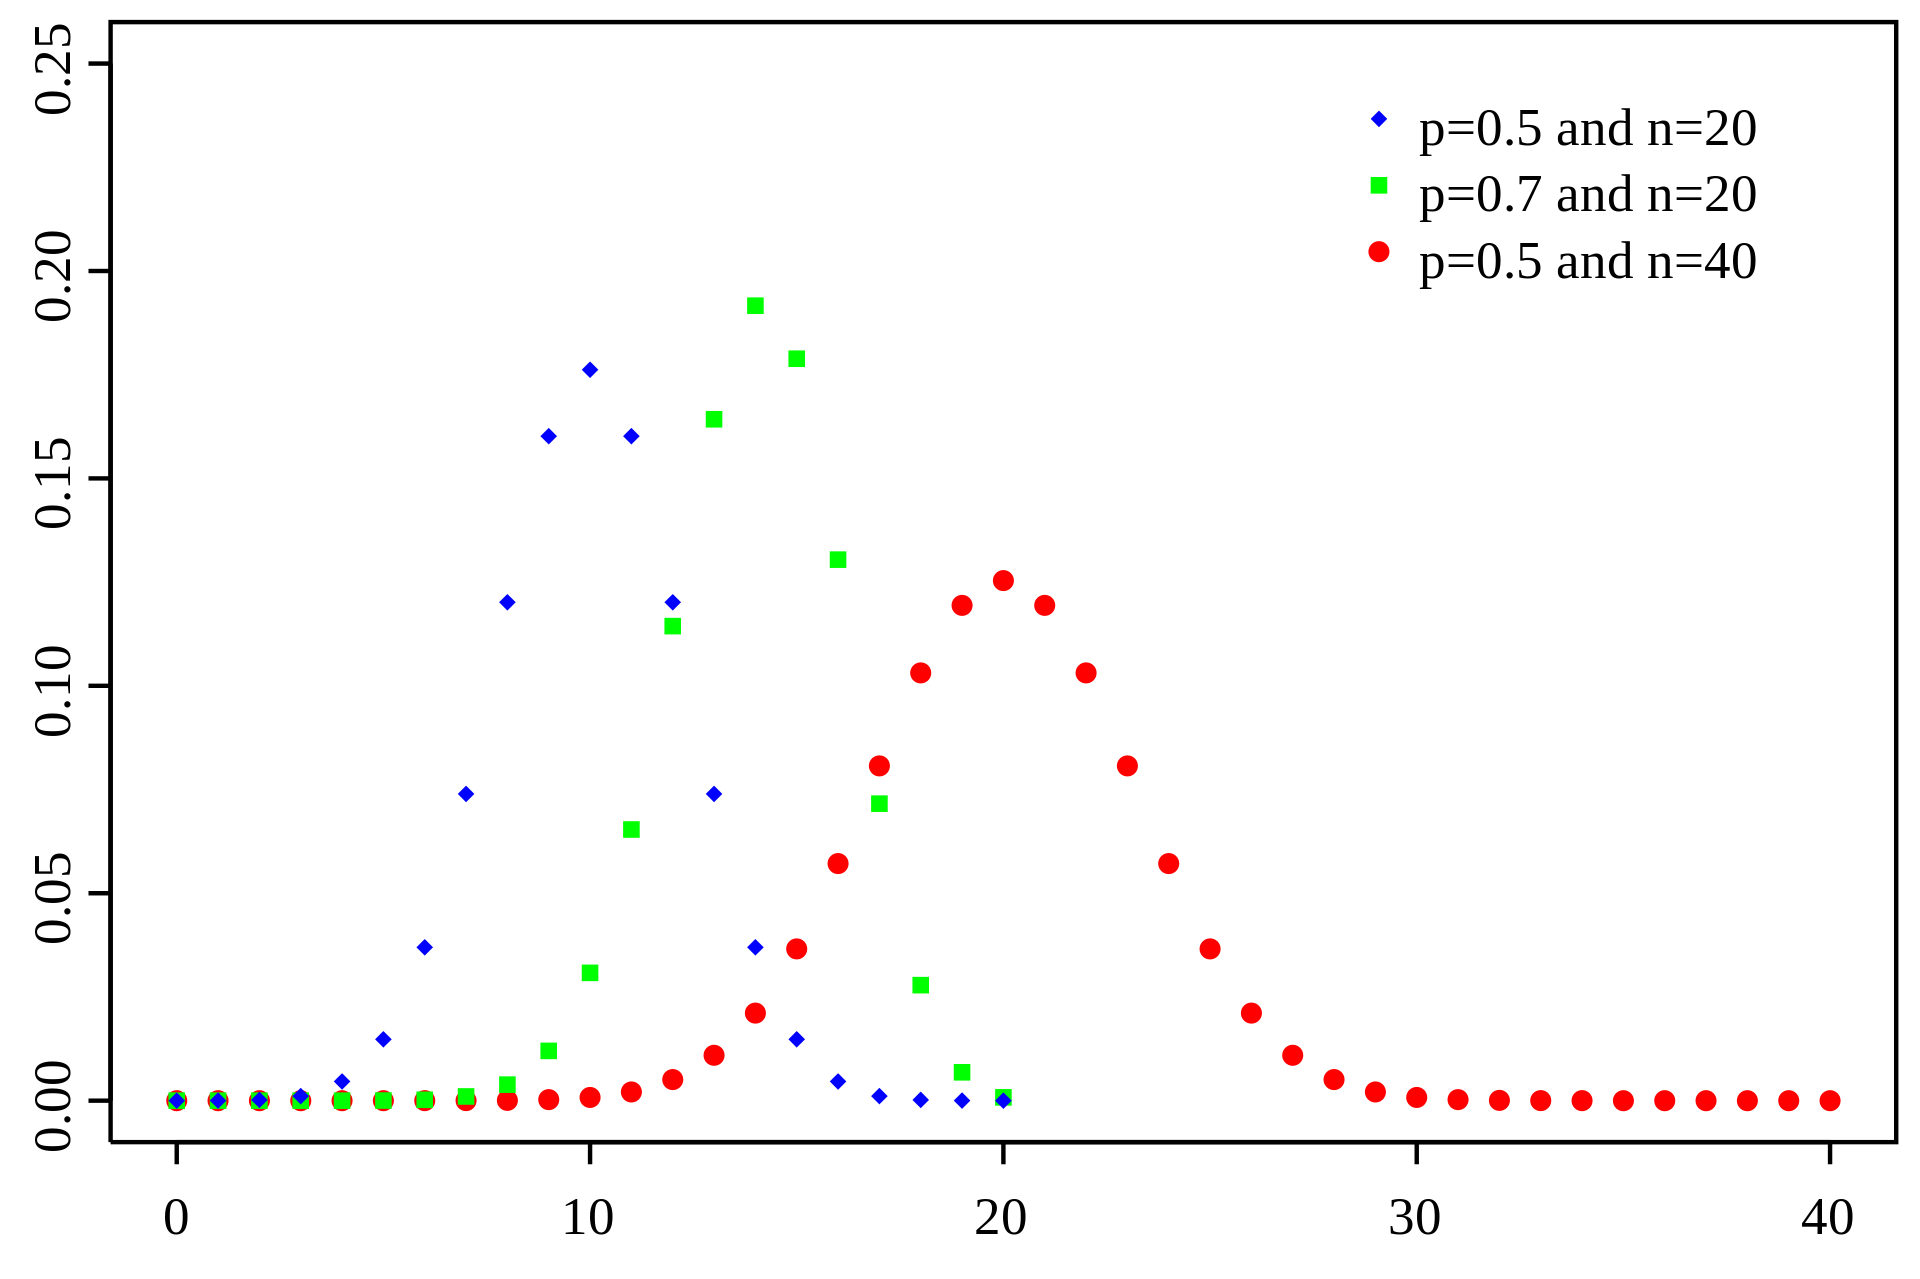
\includegraphics[scale=0.15]{1920px-Binomial_distribution_pmf.svg}
\caption{\href{https://en.wikipedia.org/wiki/Binomial_distribution}{二項分布}の確率質量関数の例}
\label{}
\end{center}
\end{figure}
\end{frame}

\begin{frame}{例. 5回のコイン投げ (1/3)}
\begin{itemize}
\item 5回のコイン投げを二項分布でモデル化する
\item コインの表と裏が出る確率は同じ1/2だとする
\item 二項分布は以下の6種類の事象の集合の上に定義される
\begin{itemize}
\item 5回のうち表が0回出る
\item 5回のうち表が1回出る
\item 5回のうち表が2回出る
\item 5回のうち表が3回出る
\item 5回のうち表が4回出る
\item 5回のうち表が5回出る
\end{itemize}
\end{itemize}
\end{frame}

\begin{frame}{例. 5回のコイン投げ (2/3)}
\begin{itemize}
\item 例えば、5回のうち表が2回出る場合は何通りあるか?
\begin{table}[t]
\Large
\begin{center}
\begin{tabular}{cccc}
11000 & 10001 & 01001 & 00011\\
10100 & 01100 & 00110 & \\
10010 & 01010 & 00101 &
\end{tabular}
\end{center}
\label{tbl:binomial_ex}
\end{table}
\vspace{-.1in}
\item 答えは、$\frac{5!}{2!3!}=10$通り
\item そして、個々の列が生起する確率は$\phi_1^2\phi_2^3=1/32$
\item よって、5回のうち表が2回出る確率は$10\times1/32=10/32$
\end{itemize}
\end{frame}

\begin{frame}{例. 5回のコイン投げ (3/3)}
\begin{itemize}
\item コインの表裏は同確率で出ると仮定している
\item よって、どんな裏表の列も、同じ$1/32$の確率で生起する
\item すると、6種類の事象のそれぞれの生起確率は、以下のようになる
\begin{itemize}
\item 5回のうち表が0回出る確率は$\frac{1}{32}$
\item 5回のうち表が1回出る確率は$\frac{5}{32}$
\item 5回のうち表が2回出る確率は$\frac{10}{32}$ ←前のスライドを参照
\item 5回のうち表が3回出る確率は$\frac{10}{32}$
\item 5回のうち表が4回出る確率は$\frac{5}{32}$
\item 5回のうち表が5回出る確率は$\frac{1}{32}$
\end{itemize}
\end{itemize}
\end{frame}


\begin{frame}
\begin{figure}[htbp]
\begin{center}
\vspace{.2in}
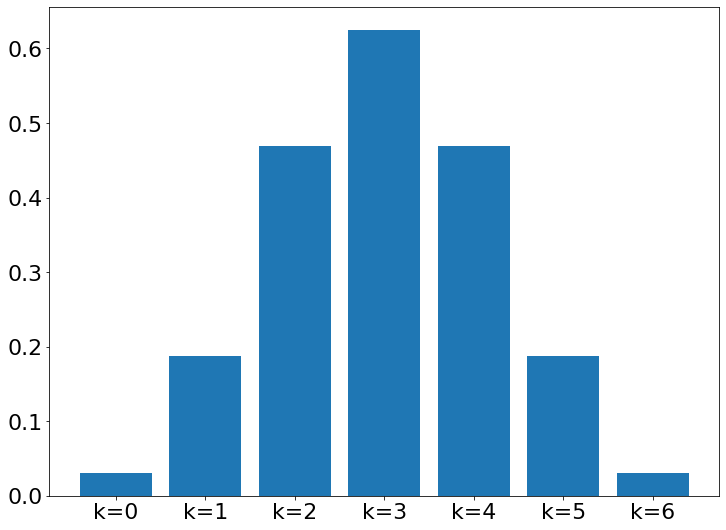
\includegraphics[scale=0.35]{binomial_bar.png}
\caption{5回のコイン投げに対応する二項分布の確率質量関数(表裏は同確率)}
\label{}
\end{center}
\end{figure}
\end{frame}


\begin{frame}{二項分布の確率質量関数}
\begin{itemize}
\item 確率質量関数 probability mass function; pmf
\begin{itemize}
\item 離散確率変数に、その値をとる確率を対応させる関数
\item 二項分布の場合は、表が出る回数にその確率を対応させる
\end{itemize}
\item 二項分布の確率質量関数
\begin{itemize}
\item $n$回の試行のうち$\mbox{v}_1$が$k$回出現する確率は:
\end{itemize}
\begin{align}
p(k;\bm{\phi},n)=\frac{n!}{k!(n-k)!}\phi_1^k\phi_2^{n-k}
\end{align}
\begin{itemize}
\item 「;」は、その右側にある$\bm{\phi}$と$n$が自由パラメータ(我々が値を定める必要があるパラメータ)であることを意味する
\end{itemize}
\end{itemize}
\end{frame}


\begin{frame}
\begin{figure}[htbp]
\begin{center}
\vspace{.2in}
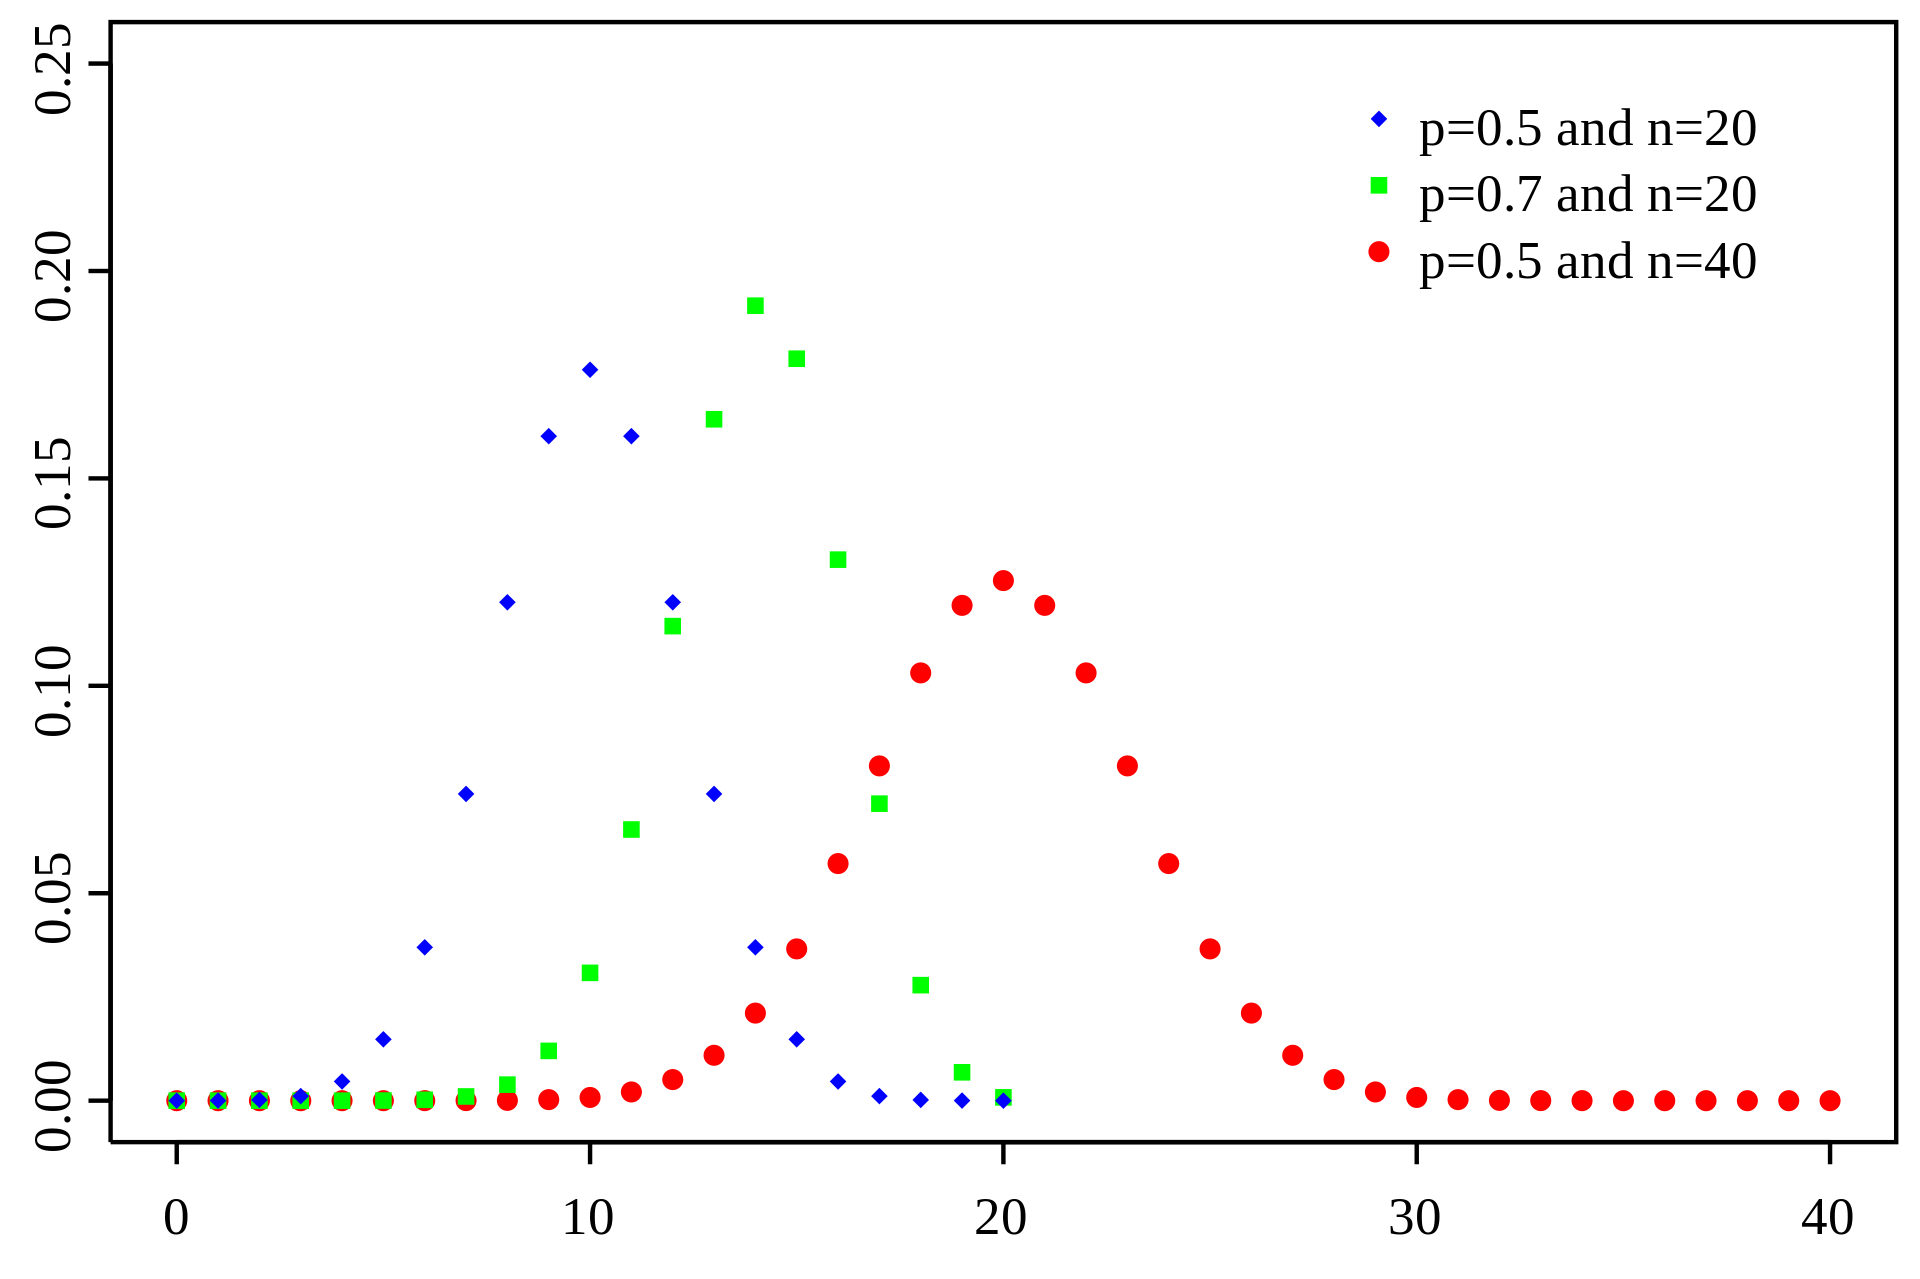
\includegraphics[scale=0.15]{1920px-Binomial_distribution_pmf.svg}
\caption{二項分布の確率質量関数の例}
\label{}
\end{center}
\end{figure}
\end{frame}


\begin{frame}{独立同分布 {\normalsize (i.i.d; independent and identically distributed)}}
\begin{itemize}
\item[] \
\vspace{-.3in}
\begin{align}
p(k;\bm{\phi},n)=\frac{n!}{k!(n-k)!}\phi_1^k\phi_2^{n-k}
\end{align}
\item 二項分布において、$n$回の試行のうちコインの表が$k$回出る確率を上の式で表すとき、以下のことを仮定している
\item[1.] 表が出る確率は履歴に左右されない
\begin{itemize}
\item 試行の独立性の仮定
\end{itemize}
\item[2.] 表が出る確率は同じままである
\begin{itemize}
\item 確率分布(この場合はベルヌーイ分布)の同一性の仮定
\end{itemize}
\item 二項分布で2種類の事象が生起する列をモデル化するとき、この仮定を置いてもいいかどうか、考える必要がある
\end{itemize}
\end{frame}

\begin{frame}{問題2-1}
\begin{itemize}
\item 表が出る確率が0.6であるコインを3回投げたとき
\begin{itemize}
\item 表が1回も出ない確率
\item 表が1回だけ出る確率
\item 表がちょうど2回出る確率
\item 3回とも表が出る確率
\end{itemize}
\item を、それぞれ求めよ。ただしi.i.d.を仮定する。
\end{itemize}
\end{frame}

\section{最尤推定}

\begin{frame}{統計モデリングの問い}
\vspace{-.5in}
\begin{block}{}
\large \center 観測されたデータを\\どのモデルが\\一番うまく説明してくれるか?
\end{block}
\vspace{.3in}
\begin{itemize}
\item 「どのモデル」
\begin{itemize}
\item モデルを選ぶ範囲をどう設定するか?
\end{itemize}
\item 「一番うまく」
\begin{itemize}
\item どういう基準でモデルを選ぶか?
\end{itemize}
\end{itemize}
\end{frame}

\begin{frame}{二項分布の場合の統計モデリングの問い}
\vspace{-.5in}
\begin{block}{}
\large \center 観測されたデータを\\
パラメータ$\phi_1$の値がいくらの二項分布が\\
一番うまく説明してくれるか?
\end{block}
\vspace{.3in}
\begin{itemize}
\item 「どのモデル」
\begin{itemize}
\item $n$が観測データの個数である二項分布のなかから選ぶ
\end{itemize}
\item 「一番うまく」
\begin{itemize}
\item まだどういう基準でモデルを選ぶかは述べられていない
\end{itemize}
\end{itemize}
\end{frame}

\begin{frame}{パラメータを使ってデータの確率を書く}
\begin{itemize}
\item 「コインを$n$回投げて表が$k$回出る確率はいくら?」
\item この問いに、二項分布によるモデリングで答えると・・・
\begin{align}
p(k;\bm{\phi},n)=\frac{n!}{k!(n-k)!}\phi_1^k\phi_2^{n-k}
\end{align}
\item パラメータを使えば、観測データが生成される確率を表せる
\item しかしパラメータは未知数
\item パラメータの値を定めること=モデルを選ぶこと
\end{itemize}
\end{frame}

\begin{frame}{観測データからパラメータを推定する}
\begin{itemize}
\item 目の前にあるこのコインを投げて表が出る確率がいくらか、分からない
\item 観測できるのは、実際にコインを投げて得られる表裏の列
\item そこで、実際にコインを投げて表が出た回数から、表が出る確率を推定estimateする
\item そのとき、観測データを「一番うまく説明してくれる」値を推定値とする
\item 「一番うまく」とは?
\end{itemize}
\end{frame}

\begin{frame}{問題2-2}
\begin{itemize}
\item コインを100回投げたら、表が52回出たとする
\item このコインの表が出る確率はいくら?
\end{itemize}
\end{frame}

\begin{frame}{問題2-2の解答例}
\begin{itemize}
\item 100回のうち表が52回出たのだから・・・
\begin{align}
\phi_1 = \frac{52}{100}
\end{align}
\item なぜこの計算でいいと考えるのか?
\begin{itemize}
\item 普通はこう計算すると思うが、なぜこう計算するのでいいと考えるのか?
\end{itemize}
\end{itemize}
\end{frame}

\begin{frame}{解答例への理屈づけ}
\begin{itemize}
\item この100回のコイン投げを二項分布でモデリングする
\begin{itemize}
\item 二項分布でモデリングすること自体は正しいのか?
\end{itemize}
\item すると、100回のうち表が52回出る、という事象の確率は
\begin{align}
p(k=52;\bm{\phi},n=100)=\frac{100!}{52!48!}\phi_1^{52}\phi_2^{48}
\end{align}
\item この式を$\phi_1$の関数とみなし、この関数を最大化する$\phi_1$の値を求めてみる
\begin{itemize}
\item $\phi_2$は$1 - \phi_1$で置き換える
\end{itemize}
\end{itemize}
\end{frame}

\begin{frame}
\begin{align}
f(\phi_1) & = \frac{100!}{52!48!}\phi_1^{52}(1-\phi_1)^{48}
\\
\frac{d f(\phi_1)}{d \phi_1} & = 
\frac{100!}{52!48!} 
\{ 52 \phi_1^{51} (1 - \phi_1)^{48} - 48 \phi_1^{52} (1 - \phi_1)^{47} \}
\notag \\ & =
\frac{100!}{52!48!} \phi_1^{51} (1 - \phi_1)^{47} \{ 52 (1 - \phi_1) - 48 \phi_1 \}
\notag \\ & =
\frac{100!}{52!48!} \phi_1^{51} (1 - \phi_1)^{47} ( 52 - 100 \phi_1 )
\label{eq:ML_derivative}
\end{align}
$\frac{d f(\phi_1)}{d \phi_1} = 0$とおくと、$\phi1=0$、$1-\phi_1=0$、$52 - 100 \phi_1 = 0$

このうち最大値が得られるのは、$\phi_1 = \frac{52}{100}$のとき。
\end{frame}

\begin{frame}{尤度 likelihood}
\vspace{-.3in}
\begin{align}
p(k=52;\bm{\phi},n=100)=\frac{100!}{52!48!}\phi_1^{52}\phi_2^{48}
\end{align}
\begin{itemize}
\vspace{-.3in}
\item 上の例のように、観測されたデータの確率を、未知数であるパラメータの関数として表したものを、尤度と呼ぶ
\item 尤度はパラメータの関数である
\begin{itemize}
\item コイン投げ100回の結果という観測データは、既知
\item つまり、観測データは定数であって、尤度はパラメータの関数
\begin{itemize}
\item パラメータの値を動かすと、尤度も動く
\end{itemize}
\end{itemize}
\end{itemize}
\end{frame}

\begin{frame}{最尤推定 maximum likelihood estimation}
\begin{itemize}
\item 式\eqref{eq:ML_derivative}のように、与えられた観測データについて尤度を最大化するパラメータの値をもってパラメータの推定値とすることを、最尤推定という
\item 尤度はパラメータの関数
\begin{itemize}
\item パラメータの値を変えると尤度が変わる、ということ
\item 観測データは既知、つまり固定された値
\end{itemize}
\end{itemize}
\end{frame}

\section{ベイズ的な考え方}

\begin{frame}\frametitle{Contents}
\Large \tableofcontents[currentsection]
\end{frame}

\begin{frame}{問題2-2の解答例(再び)}
\begin{itemize}
\item 100回のうち表が52回出たのだから・・・
\begin{align}
\phi_1 = \frac{52}{100}
\end{align}
\item しかし…この求め方で本当にいいのか?
\item ダメだとすればその理由は?
\item[] \
\item 表が出る確率を、その100回のコイン投げだけで決めてしまっていいのか?
\end{itemize}
\end{frame}

\begin{frame}{ベイズ的な考え方}
\begin{itemize}
\item 表が出る確率を決めること自体に不確かさがある、と考える
\item つまり、$\phi_1$が$0$から$1$のあいだのどの値をとるかも確率的に決まる、と考える
\item 言い換えれば、パラメータもまた確率変数だと考える
\begin{itemize}
\item これがベイズ的な考え方
\end{itemize}
\item つまり、ベイズ的なデータのモデル化は二段構え
\begin{itemize}
\item[1.] コイン投げで表が何回出るかは確率的に決まる
\item[2.] それだけでなく、表が出る確率も確率的に決まる
\end{itemize}
\end{itemize}
\end{frame}

\begin{frame}{パラメータの値が確率的に決まるとは?}
\begin{itemize}
\item 表が出る確率$\phi_1$は様々でありうる
\begin{itemize}
\item 0.01, 0.1, 0.3, 0.6, 0.98等々・・・0以上1以下なら何でもOK
\end{itemize}
\item とびとびの値ではなく連続的な値
\begin{itemize}
\item 表が出る確率の値が何通りあるかなんて言えない
\begin{itemize}
\item 強いて言えば、無限通りある
\end{itemize}
\end{itemize}
\item つまり、0から1までの連続的な値それぞれをとる確率を考える必要がある
\item 言い換えれば、区間$[0,1]$上に定義される連続確率分布を考える必要がある
\end{itemize}
\end{frame}

\begin{frame}{連続確率分布}
\vspace{.25in}
\begin{itemize}
\item 連続分布は確率密度関数probability density function (pdf)で表すことが多い(例. 右図は正規分布の場合)
\item 確率密度関数は、定義域全域で積分すると1になる
\item 連続分布を累積密度関数cumulative distribution function (cdf)で表すこともある
\begin{itemize}
\item ざっくり言えば、pdfを積分するとcdf
\begin{align}
F(x) = \int_{-\infty}^x f(t) dt
\end{align}
\end{itemize}
\end{itemize}
\begin{textblock*}{0.4\linewidth}(300pt, 7pt)
    \centering
    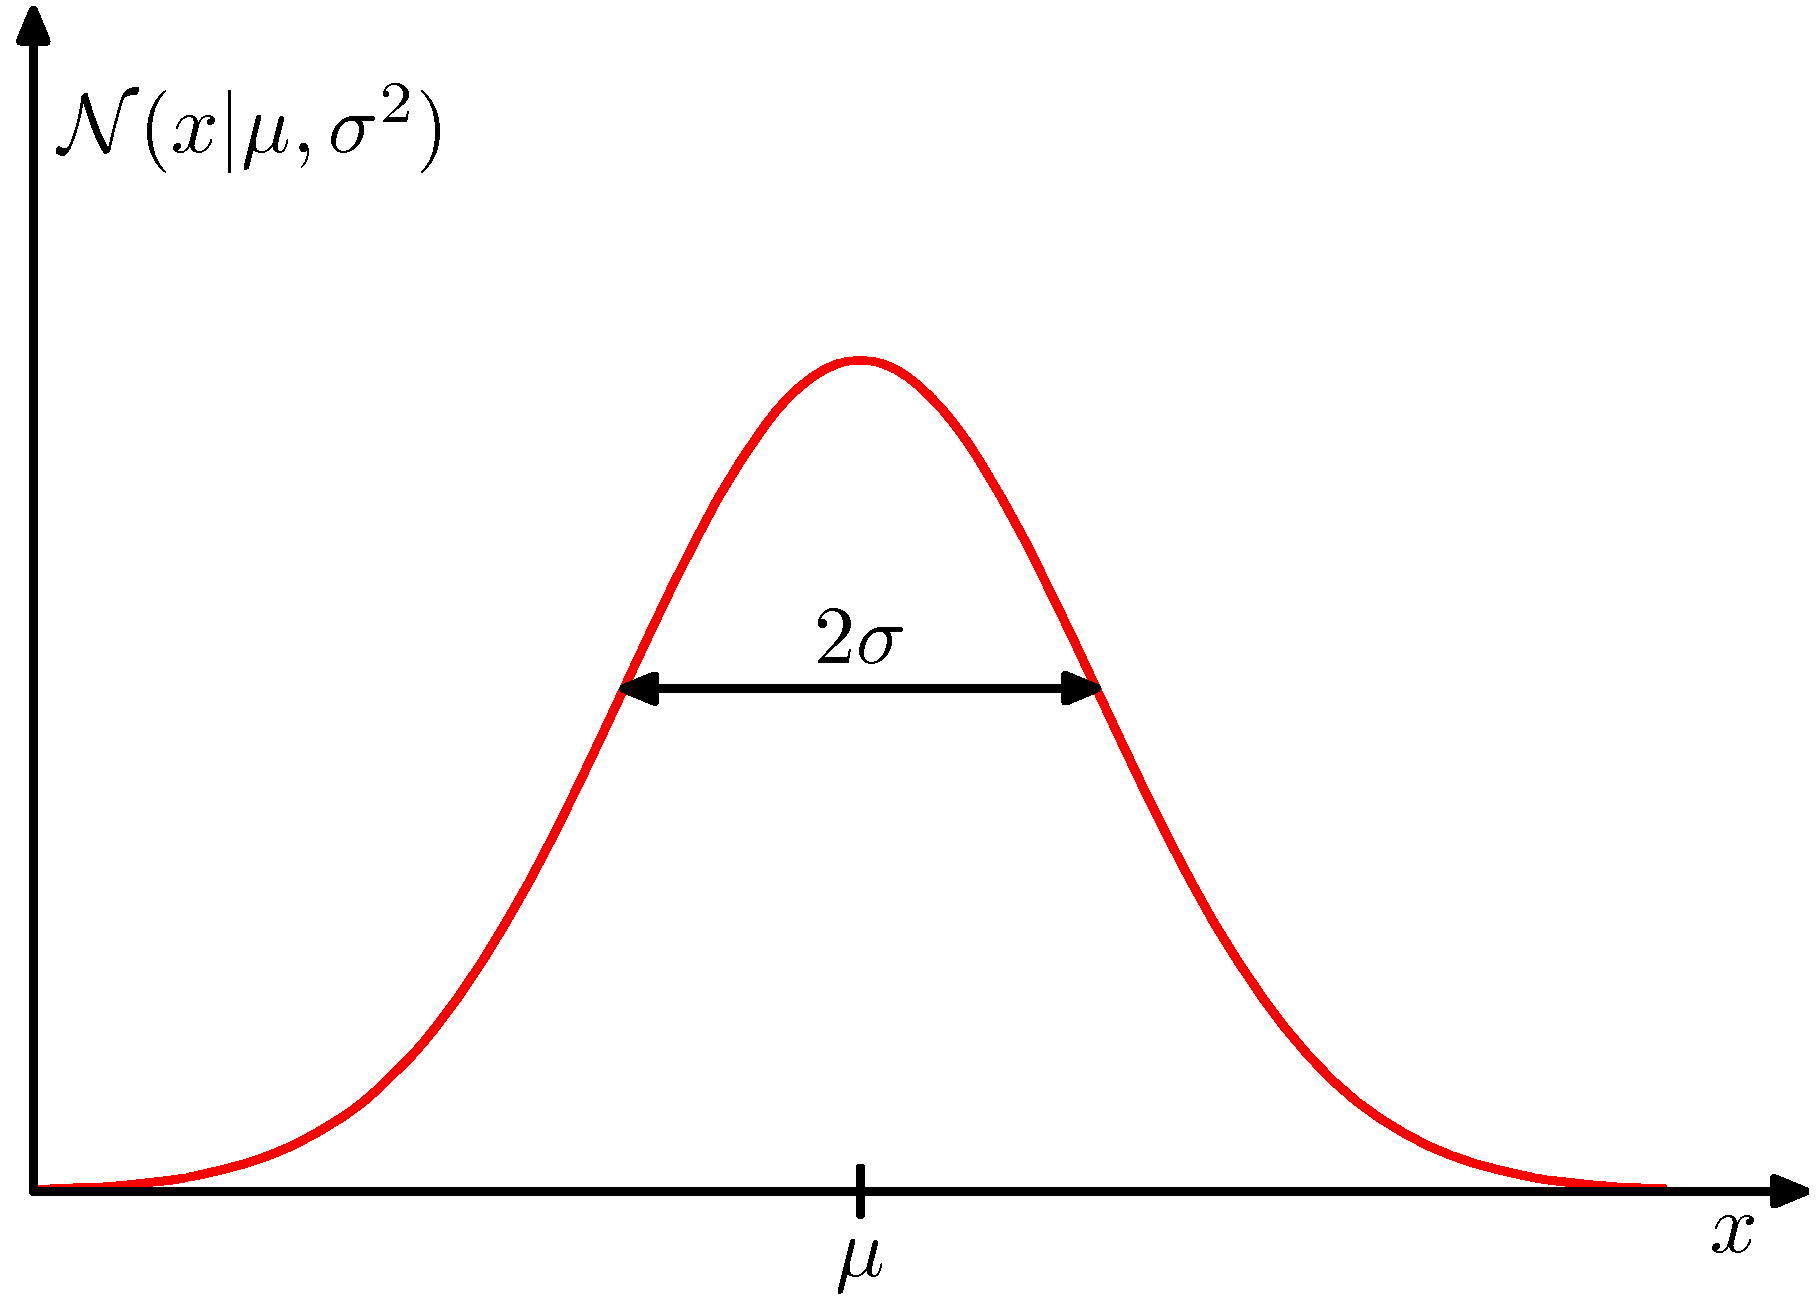
\includegraphics[width=0.5\linewidth]{Figure1.13.png}
\end{textblock*}
\begin{textblock*}{0.4\linewidth}(300pt, 170pt)
    \centering
    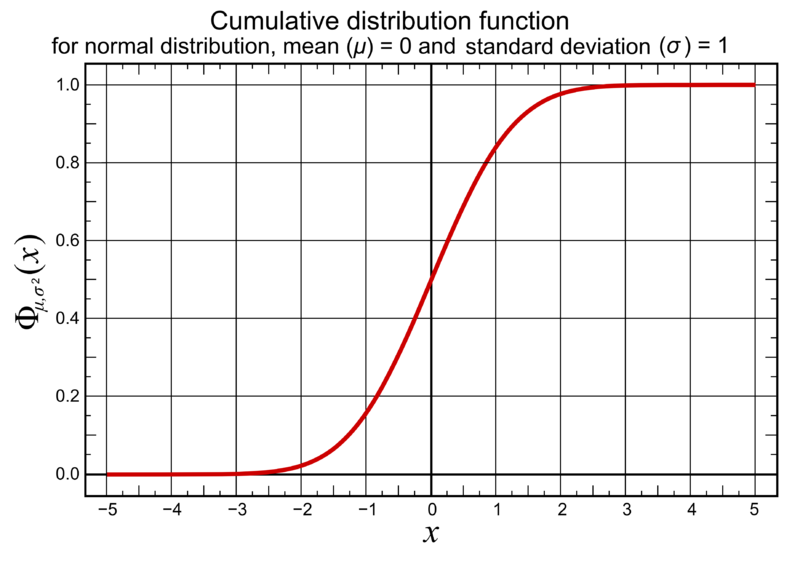
\includegraphics[width=0.6\linewidth]{800px-Cumulative_distribution_function_for_normal_distribution,_mean_0_and_sd_1.png}
\end{textblock*}
\end{frame}


\begin{frame}{一様分布}
\begin{itemize}
\item 連続値に確率を定める確率分布のひとつの例
\item 定義域はいろいろでありうる
\begin{itemize}
\item コインの表が出る確率$\phi_1$の場合は$[0,1]$の範囲
\end{itemize}
\end{itemize}
\begin{figure}[htbp]
\begin{center}
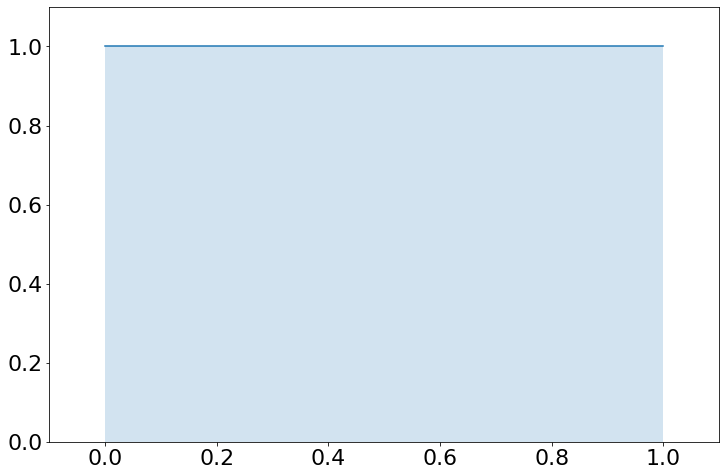
\includegraphics[scale=0.27]{uniform_dist.png}
\vspace{-.2in}
\caption{区間$[0,1]$上の一様分布}
\label{}
\end{center}
\end{figure}
\end{frame}

\begin{frame}{復習:ベイズ則}
\vspace{-.4in}
{\Large
\begin{align}
p(z|x) \propto p(x|z)p(z)
\notag
\end{align}
}%
\vspace{-.2in}
\begin{itemize}
\item ある仮説が成り立つ確率$p(z)$は・・・
\item その仮説が成り立つときに尤もらしさ$p(x|z)$が大きいデータ$x$が観測されると・・・
\item 高い値の確率$p(z|x)$になる
\end{itemize}
\end{frame}

\begin{frame}{ベイズ則をベイズ的なモデリングで使う}
\vspace{-.4in}
{\Large
\begin{align}
p(\theta|x) \propto p(x|\theta)p(\theta)
\end{align}
}%
\vspace{-.2in}
\begin{itemize}
\item モデルのパラメータ$\theta$がある値をとる確率$p(\theta)$は・・・
\item パラメータがその値をとるときに尤度$p(x|\theta)$が大きいデータ$x$が観測されると・・・
\item 高い値の確率$p(\theta|x)$になる
\end{itemize}
\end{frame}

\section{実践:コイン投げのベイズ的モデル化}

\begin{frame}\frametitle{Contents}
\Large \tableofcontents[currentsection]
\end{frame}

\begin{frame}{一様分布からスタートする}
\begin{itemize}
\item コインの表が出る確率がいくらかなんて全く分からないという状態からスタートすることにする
\begin{itemize}
\item 常識的には「ほぼ1/2」と仮定するのが自然だが、今回はこうする
\end{itemize}
\item そこで、表が出る確率$\phi_1$が区間$[0,1]$のどの値をとるかについては、一様分布を仮定することにする
\item つまり、$p(\phi_1)=1$と仮定する
\begin{itemize}
\item これは、$\phi_1$がどの値をとることも全く同じようにありえそう、という意味
\end{itemize}
\end{itemize}
\begin{textblock*}{0.4\linewidth}(300pt, 3pt)
    \centering
    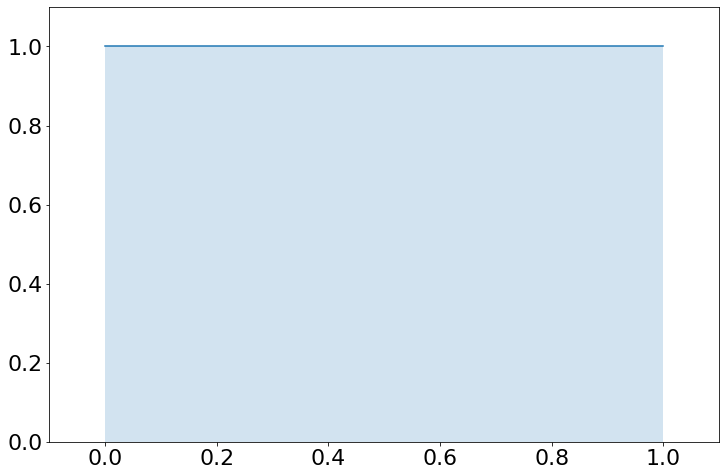
\includegraphics[width=0.5\linewidth]{uniform_dist.png}
\end{textblock*}
\end{frame}

\begin{frame}{1回コインを投げたら表だったとする}
\vspace{-.3in}
\begin{align}
p(\phi_1 | x_1 = \mbox{H}) \propto p(x_1 = \mbox{H} | \phi_1) p(\phi_1)
\notag
\end{align}
$p(\phi_1)$は一様分布だと仮定したので、$p(\phi_1)=1$。また、
尤度$p(x_1 = \mbox{H} | \phi_1)$は$\phi_1$に等しい。
よって、
\begin{align}
p(\phi_1 | x_1 = \mbox{H}) \propto \phi_1 \times 1 = \phi_1
\end{align}
右辺を規格化する。つまり、$[0,1]$で積分して1になるようにする。
$\int_0^1 \phi_1 d\phi_1 = \Big[ \frac{\phi_1^2}{2} \Big]_0^1 = \frac{1}{2}$より、
右辺を$\frac{1}{2}$で割って
\begin{align}
p(\phi_1 | x_1 = \mbox{H}) = 2\phi_1
\end{align}
\end{frame}

\begin{frame}
\begin{textblock*}{0.4\linewidth}(20pt, 30pt)
    \centering
    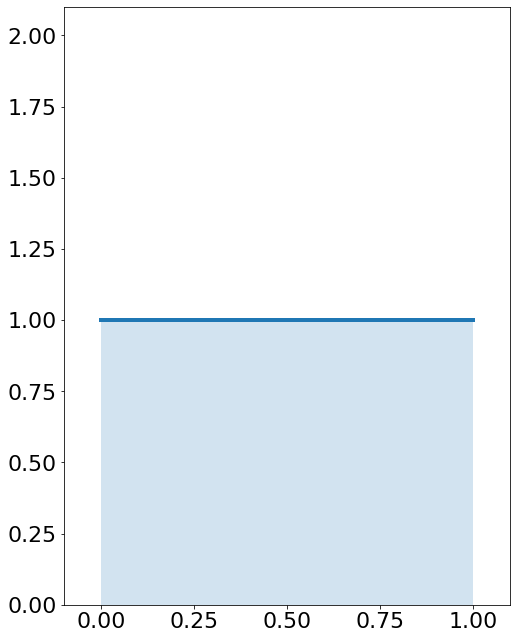
\includegraphics[width=\linewidth]{beta_1_1.png}
\end{textblock*}
\begin{textblock*}{0.4\linewidth}(145pt, 110pt)
    \centering
    
\includegraphics[width=0.3\linewidth]{blue_arrow.png}
\end{textblock*}
\begin{textblock*}{0.4\linewidth}(270pt, 30pt)
    \centering
    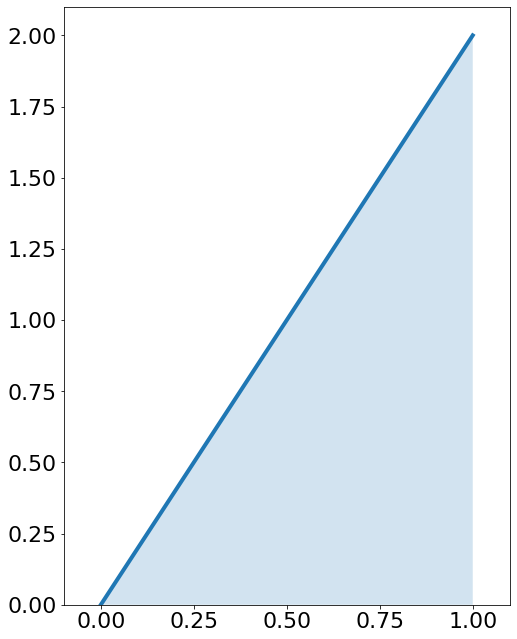
\includegraphics[width=\linewidth]{beta_2_1.png}
\end{textblock*}
\end{frame}

\begin{frame}{もう1回コインを投げたら裏だったとする}
\vspace{-.3in}
\begin{align}
p(\phi_1 | x_1 = \mbox{H}, x_2 = \mbox{T}) 
\propto p(x_1 = \mbox{H}, x_2 = \mbox{T} | \phi_1) p(\phi_1)
\notag
\end{align}
$p(\phi_1)$は一様分布だと仮定したので、$p(\phi_1)=1$。また、
尤度$p(x_1 = \mbox{H}, x_2 = \mbox{T} | \phi_1)$は$\phi_1(1-\phi_1)$に等しい。
よって、
\begin{align}
p(\phi_1 | x_1 = \mbox{H}, x_2 = \mbox{T}) \propto \phi_1(1-\phi_1)
\end{align}
右辺を規格化する。つまり、$[0,1]$で積分して1になるようにする。
$\int_0^1 \phi_1(1-\phi_1) d\phi_1 = \Big[ \frac{\phi_1^2}{2} - \frac{\phi_1^3}{3} \Big]_0^1= \frac{1}{6}$より、
右辺を$\frac{1}{6}$で割って
\begin{align}
p(\phi_1 | x_1 = \mbox{H}, x_2 = \mbox{T}) = 6\phi_1(1-\phi_1)
\end{align}
\end{frame}

\begin{frame}
\begin{textblock*}{0.4\linewidth}(20pt, 30pt)
    \centering
    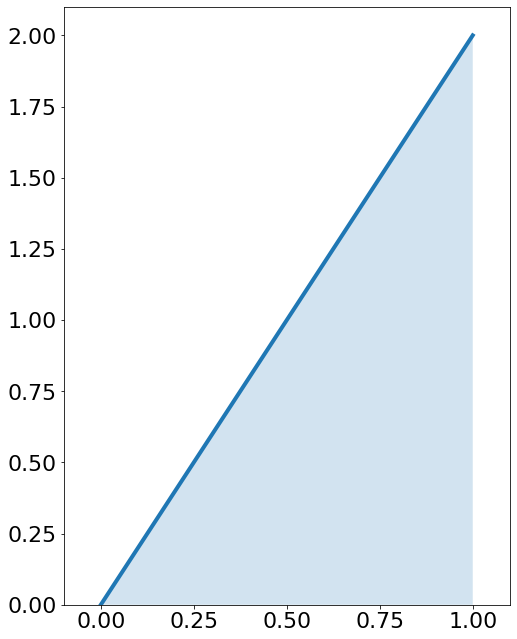
\includegraphics[width=\linewidth]{beta_2_1.png}
\end{textblock*}
\begin{textblock*}{0.4\linewidth}(145pt, 110pt)
    \centering
    
\includegraphics[width=0.3\linewidth]{blue_arrow.png}
\end{textblock*}
\begin{textblock*}{0.4\linewidth}(270pt, 30pt)
    \centering
    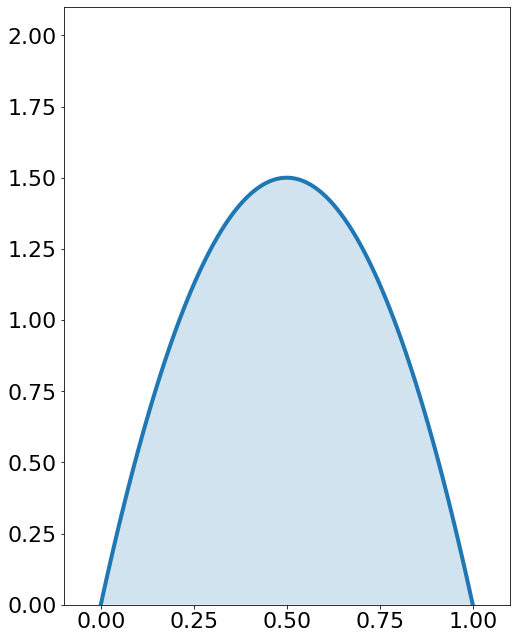
\includegraphics[width=\linewidth]{beta_2_2.png}
\end{textblock*}
\end{frame}

\begin{frame}{もう1回コインを投げたら表だったとする}
\vspace{-.3in}
\begin{align}
p(\phi_1 | x_1 = \mbox{H}, x_2 = \mbox{T}, x_3 = \mbox{H}) 
\propto p(x_1 = \mbox{H}, x_2 = \mbox{T}, x_3 = \mbox{H} | \phi_1) p(\phi_1)
\notag
\end{align}
$p(\phi_1)$は一様分布だと仮定したので、$p(\phi_1)=1$。また、
尤度$p(x_1 = \mbox{H}, x_2 = \mbox{T}, x_3 = \mbox{H} | \phi_1)$は$\phi_1^2(1-\phi_1)$に等しい。
よって、
\begin{align}
p(\phi_1 | x_1 = \mbox{H}, x_2 = \mbox{T}, x_3 = \mbox{H}) \propto \phi_1^2(1-\phi_1)
\end{align}
右辺を規格化する。つまり、$[0,1]$で積分して1になるようにする。
$\int_0^1 \phi_1^2(1-\phi_1) d\phi_1 =\Big[ \frac{\phi_1^3}{3} - \frac{\phi_1^4}{4} \Big]_0^1= \frac{1}{12}$より、
右辺を$\frac{1}{12}$で割って
\begin{align}
p(\phi_1 | x_1 = \mbox{H}, x_2 = \mbox{T}, x_3 = \mbox{H}) = 12\phi_1^2(1-\phi_1)
\end{align}
\end{frame}

\begin{frame}
\begin{textblock*}{0.4\linewidth}(20pt, 30pt)
    \centering
    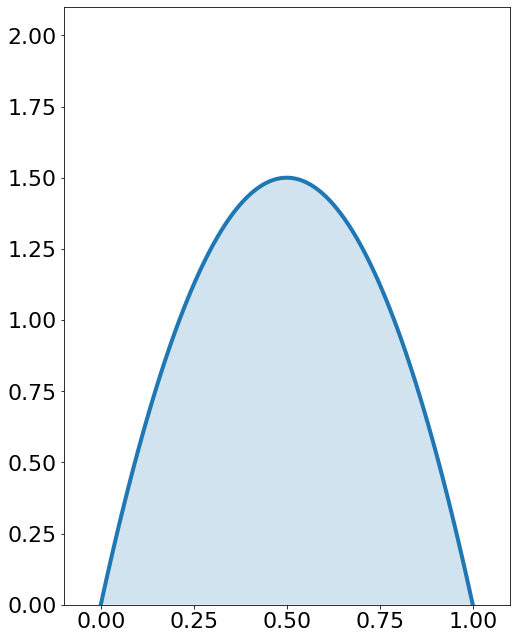
\includegraphics[width=\linewidth]{beta_2_2.png}
\end{textblock*}
\begin{textblock*}{0.4\linewidth}(145pt, 110pt)
    \centering
    
\includegraphics[width=0.3\linewidth]{blue_arrow.png}
\end{textblock*}
\begin{textblock*}{0.4\linewidth}(270pt, 30pt)
    \centering
    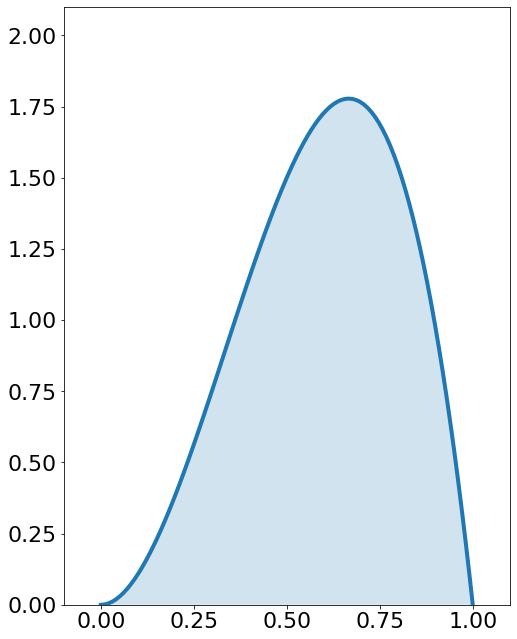
\includegraphics[width=\linewidth]{beta_3_2.png}
\end{textblock*}
\end{frame}

\begin{frame}{結局、合計100回投げたら表が52回出たとする}
\begin{figure}[htbp]
\begin{center}
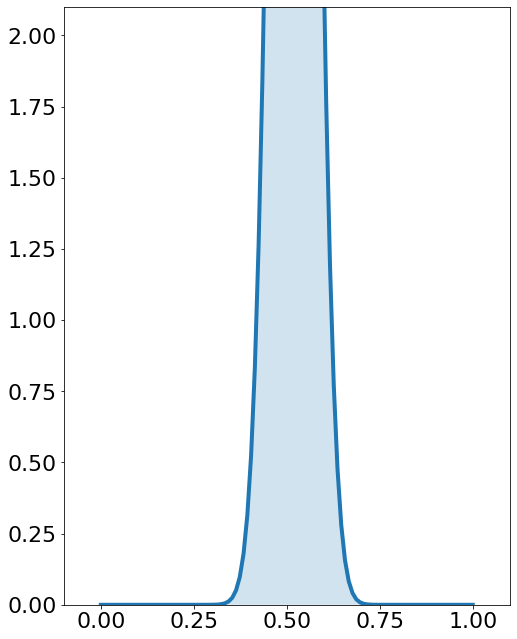
\includegraphics[scale=0.3]{beta_53_49.png}
\caption{一様分布からスタート、合計100回投げたら表が52回出た}
\label{}
\end{center}
\end{figure}
\end{frame}

\begin{frame}{問題2-2の先ほどの解答例との違い}
\begin{adjustwidth}{0em}{4em}
\begin{itemize}
\item 「合計100回投げて表が52回出た」という出題に、最初の解答例では52/100と答えを求めていた
\item 今回は、連続的な関数(右図)で答えている
\begin{itemize}
\item 表が出る確率として考えられる0から1の値について、それぞれがどのくらいありえそうかで、答えている
\item 答えをひとつの値に決めていない、とも言える
\end{itemize}
\end{itemize}
\end{adjustwidth}
\begin{textblock*}{0.4\linewidth}(330pt, 70pt)
    \centering
    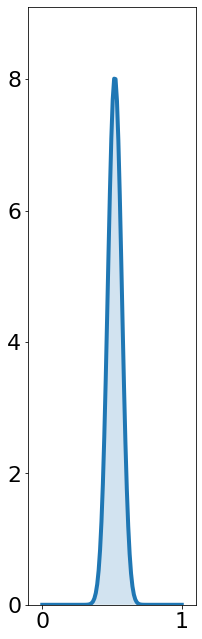
\includegraphics[scale=0.25]{beta_53_49_L.png}
\end{textblock*}
\end{frame}

\begin{frame}{ベータ分布 beta distribution}
\begin{itemize}
\item 上の説明に出てきた連続分布をベータ分布と呼ぶ
\item ベータ分布は、2つのパラメータ$a$と$b$を持つ
\item 確率密度関数は以下の式
{\Large
\begin{align}
p(x;a,b) = \frac{\Gamma(a+b)}{\Gamma(a)\Gamma(b)}x^{a-1}(1-x)^{b-1}
\notag
\end{align}
}%
\begin{itemize}
\item $\frac{\Gamma(a+b)}{\Gamma(a)\Gamma(b)}$は、規格化定数
\end{itemize}
\end{itemize}
\end{frame}

\begin{frame}{事前分布と事後分布}
\begin{itemize}
\item 事前分布 prior distribution
\begin{itemize}
\item 今日の話では、最初にそこからスタートしたところの一様分布が、事前分布
\end{itemize}
\item 事後分布 posterior distribution
\begin{itemize}
\item 今日の話でそのつど求めていた$p(\phi_1 | \bm{x})$が、事後分布
\end{itemize}
\item ベイズ的な統計モデリングでは、観測データにもとづいて事後分布を求めることが、主な課題!
\end{itemize}
\end{frame}

\begin{frame}{ベイズ的モデリングにおけるベイズ則}
\begin{itemize}
\item ベイズ推論で使うベイズ則は、単に条件付き確率どうしの関係を表すだけの式ではない
\end{itemize}
{\Large
\begin{align}
\mbox{(事後分布)} \propto \mbox{(尤度)} \times \mbox{(事前分布)}
\notag
\end{align}
}%
\vspace{-.2in}
\begin{itemize}
\item 上の式が、ベイズ的な統計モデリング特有のベイズ則の使い方
\end{itemize}
\end{frame}

\begin{frame}{課題2}
\begin{itemize}
\item $\phi$の関数$f(\phi)=\phi^3(1-\phi)^2$を$[0,1]$の範囲で積分せよ。
\item 積分した結果が$1$になるようにするためには、$f(\phi)$にいくらを掛けておけばよかったか。
\end{itemize}
\end{frame}

\end{document}